\chapter{Post-Flight Simulation Thermal Properties}\label{post_flight_thermal_properties_appendix}

The purpose of this appendix is to provide all thermal inputs and settings used in the final simulations of the LIFE model. Using the following properties, the LIFE thermal simulations can be exactly reproduced, given the LIFE CAD model. These tables are output from SolidWorks automatically for this purpose. An explanation of these tables and how they are interpreted is described here.

The tables are split into two colours, red and blue. The red tables describe all heat loads, such as radiation and power, and have four columns: load name, load image, load detail, and function curve. Load name describes the part in question as a variable name in the simulation, i.e. BB{\textunderscore}Temp{\textunderscore}Controllers would be the temperature controllers of the blackbody electronics box. The load image shows a screenshot of the model, with the affected areas (i.e. the surface of radiation, or the part emitting power) highlighted in blue. The third column, load details, describes all settings for that particular load set in the simulation. Finally, if applicable the fourth column is the function curve, which will show the radiation or heat power changing with time if it is a transient load. This box is blank if the load is steady-state.

The blue tables describe custom contacts between parts, and are split into three columns: contact, contact image, and contact properties. The first column describes the name of the joint as a variable name. The second column is a screenshot showing the two surfaces that make contact, with one surface highlighted in blue and the other highlighted in purple. One surface may be hard to see in the image if it is facing away from view. The final column describes settings of the joint in question, most notably the thermal resistance value. For all part contacts not contained in the blue tables, it is assumed to be a bonded contact.

It is hoped that these heat loads will provide insight into the thermal simulations of LIFE and can be used to inform future instrument thermal models, and can also be used if anything happens to the thermal model file of LIFE.

\newpage

\section{Ascent Phase: Part 1}

\begin{figure}[h!]
    \centering
    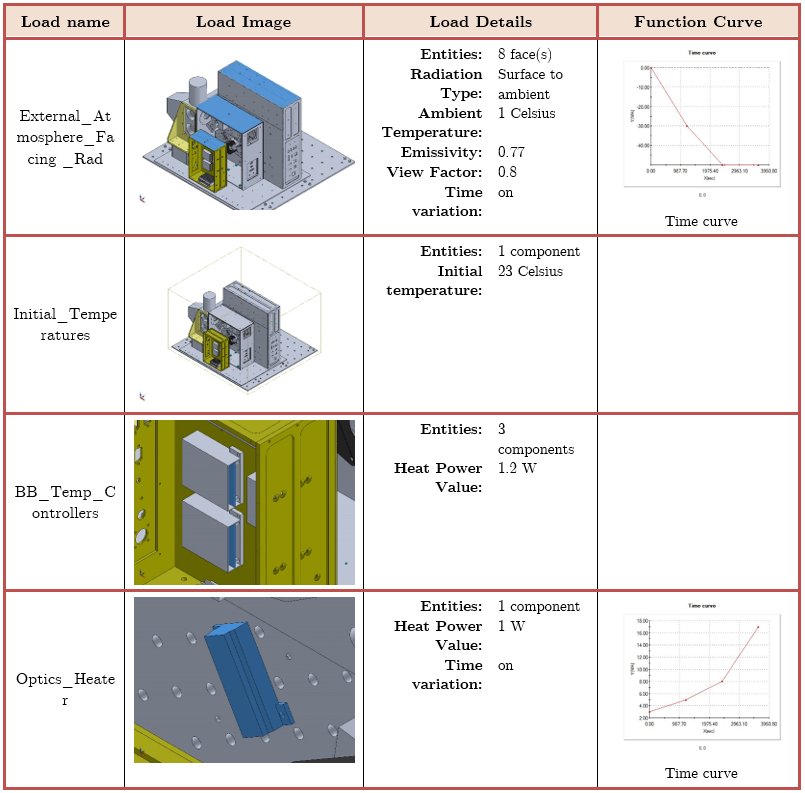
\includegraphics[width=\textwidth]{thermal_load_images/ascent_pt1_TL_images/ascesnt_pt1_1.PNG}
\end{figure}

\begin{figure}
    \centering
    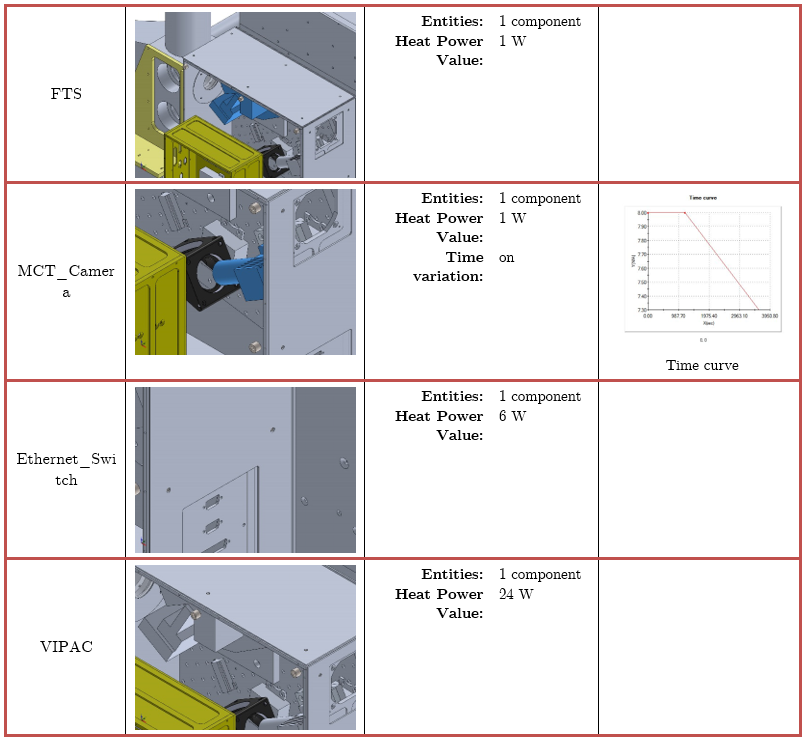
\includegraphics[width=\textwidth]{thermal_load_images/ascent_pt1_TL_images/ascesnt_pt1_2.png}
\end{figure}

\begin{figure}
    \centering
    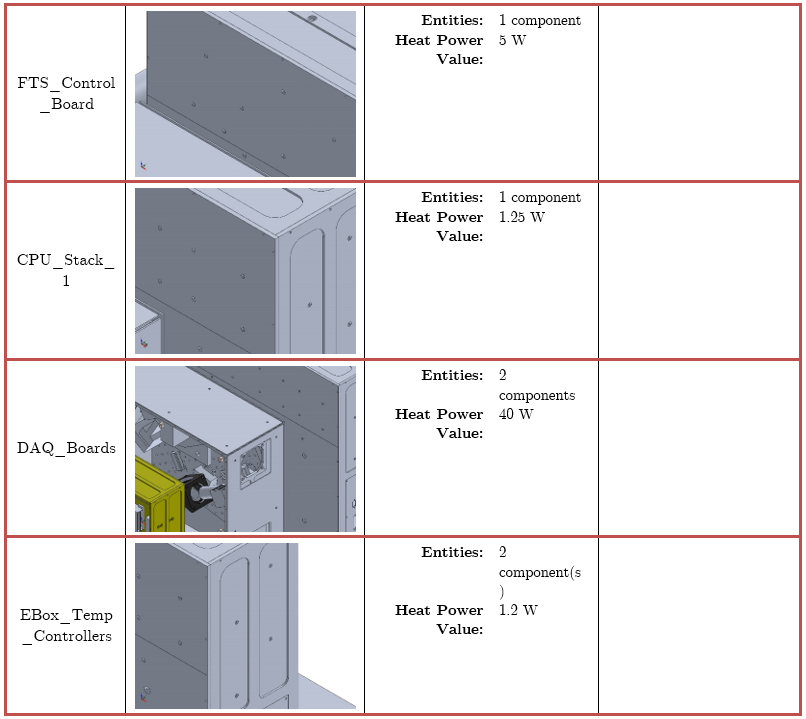
\includegraphics[width=\textwidth]{thermal_load_images/ascent_pt1_TL_images/ascesnt_pt1_3.PNG}
\end{figure}

\begin{figure}
    \centering
    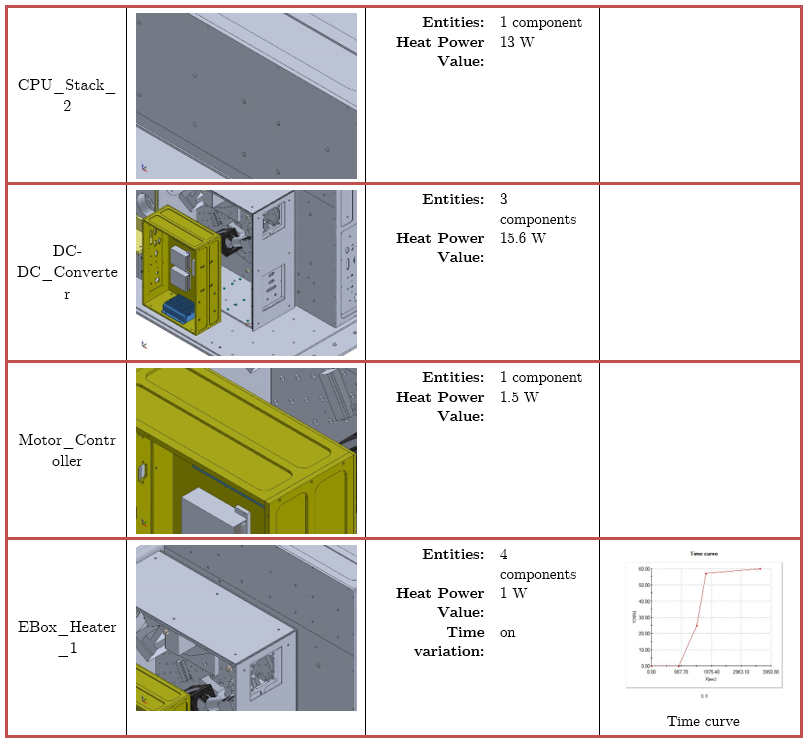
\includegraphics[width=\textwidth]{thermal_load_images/ascent_pt1_TL_images/ascesnt_pt1_4.PNG}
\end{figure}

\begin{figure}
    \centering
    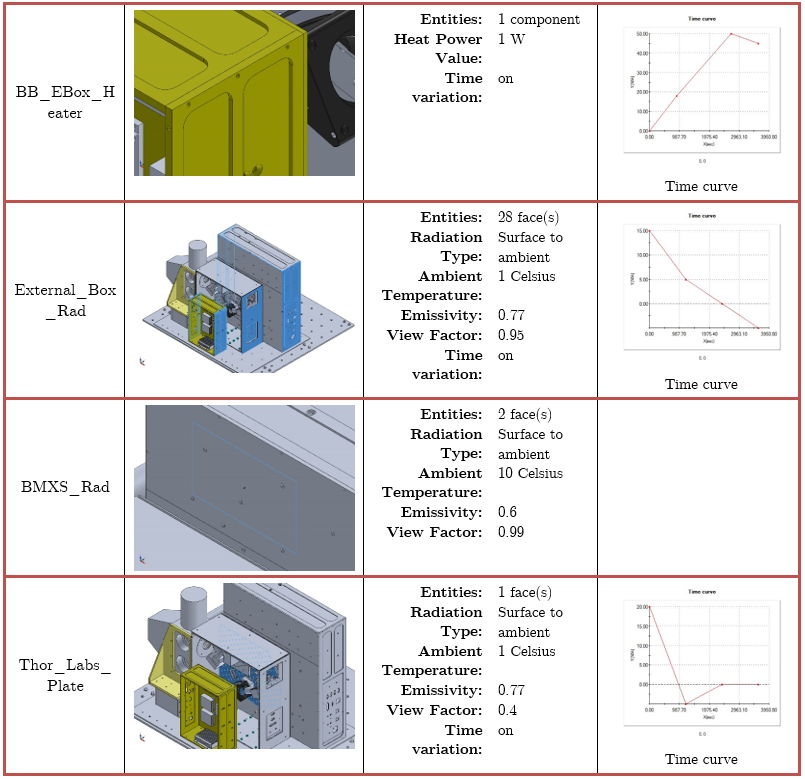
\includegraphics[width=\textwidth]{thermal_load_images/ascent_pt1_TL_images/ascesnt_pt1_5.PNG}
\end{figure}

\begin{figure}
    \centering
    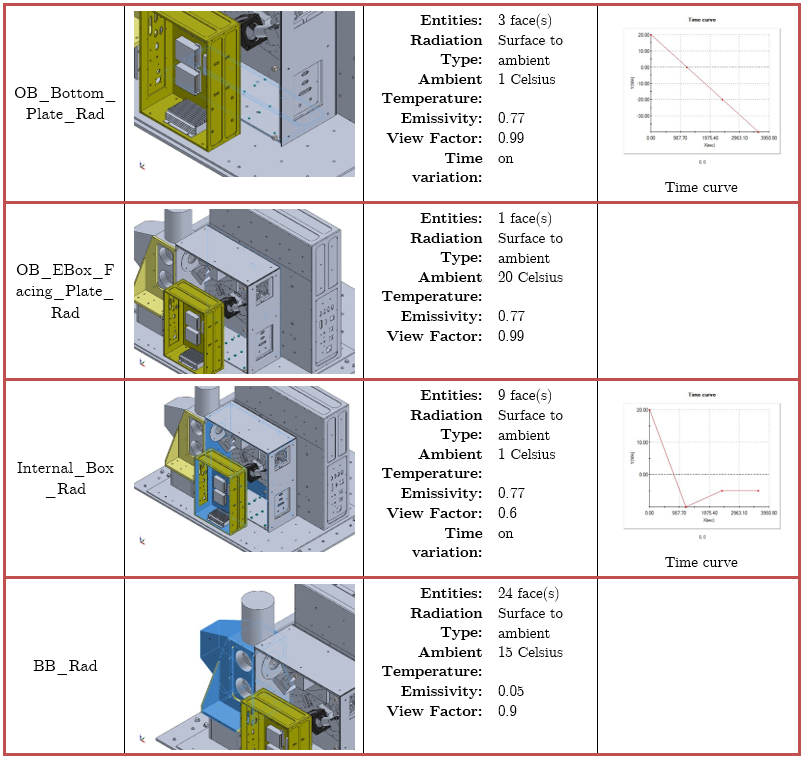
\includegraphics[width=\textwidth]{thermal_load_images/ascent_pt1_TL_images/ascesnt_pt1_6.PNG}
\end{figure}

\begin{figure}
    \centering
    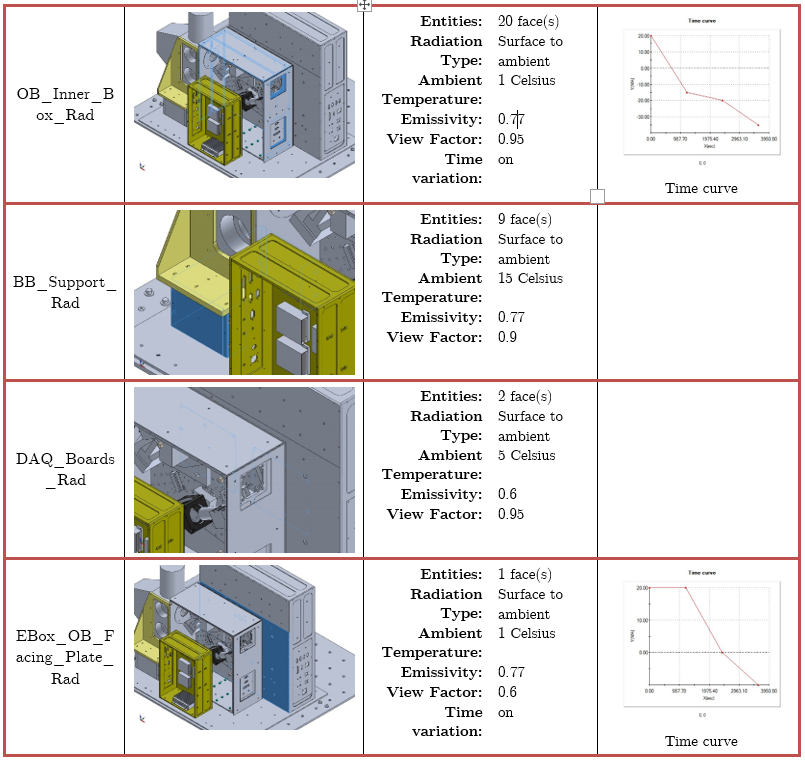
\includegraphics[width=\textwidth]{thermal_load_images/ascent_pt1_TL_images/ascesnt_pt1_7.PNG}
\end{figure}

\begin{figure}
    \centering
    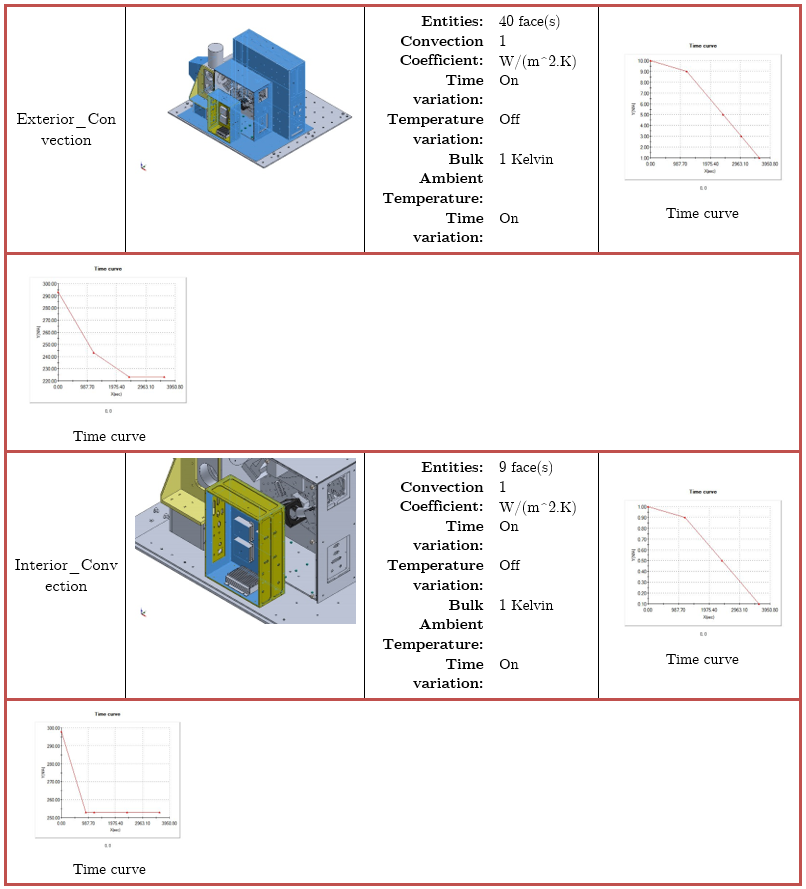
\includegraphics[width=\textwidth]{thermal_load_images/ascent_pt1_TL_images/ascesnt_pt1_8.PNG}
\end{figure}

\begin{figure}
    \centering
    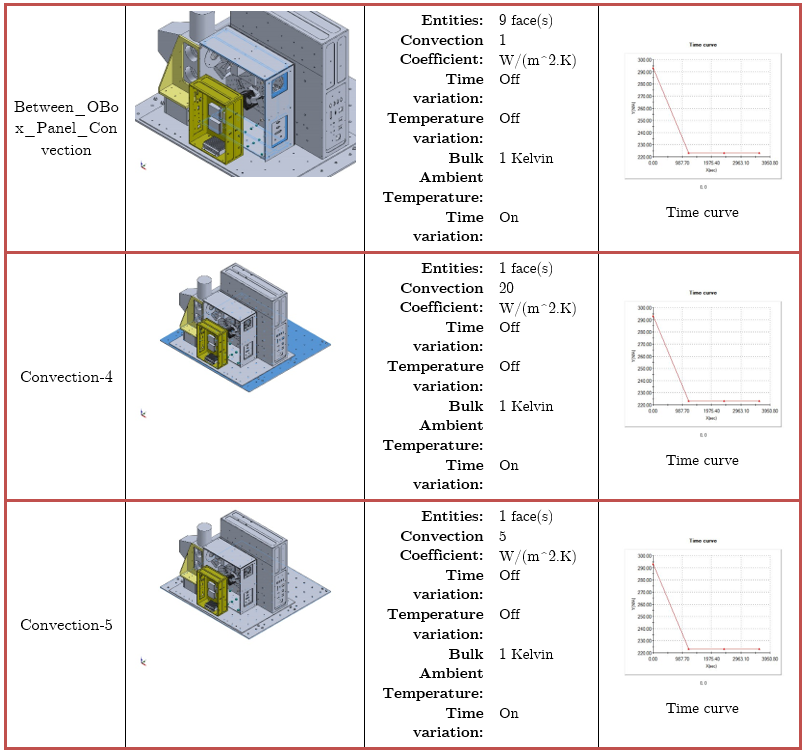
\includegraphics[width=\textwidth]{thermal_load_images/ascent_pt1_TL_images/ascesnt_pt1_9.PNG}
\end{figure}

\begin{figure}
    \centering
    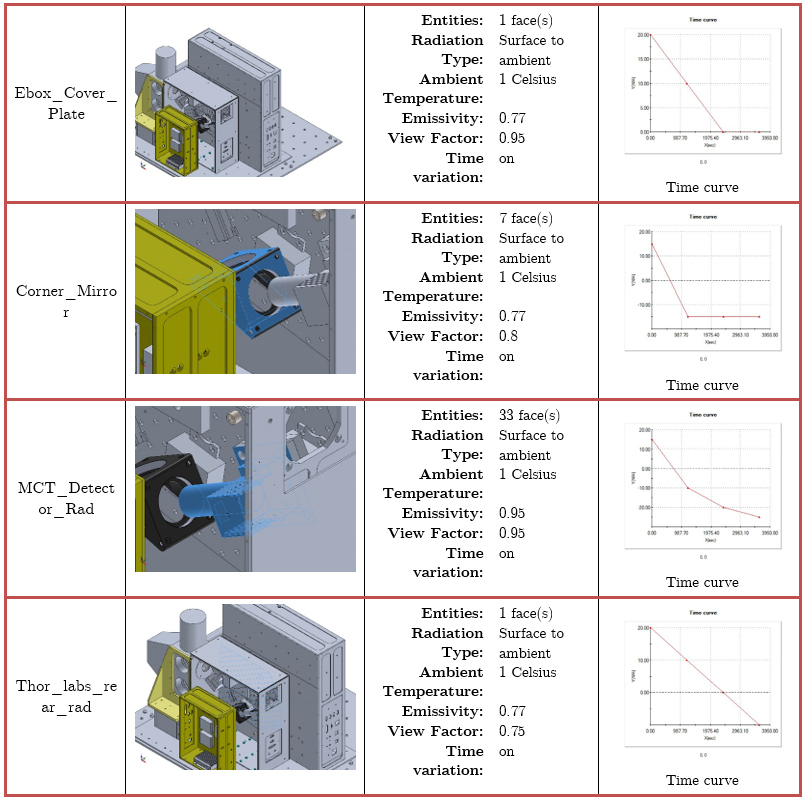
\includegraphics[width=\textwidth]{thermal_load_images/ascent_pt1_TL_images/ascesnt_pt1_10.PNG}
\end{figure}

\begin{figure}
    \centering
    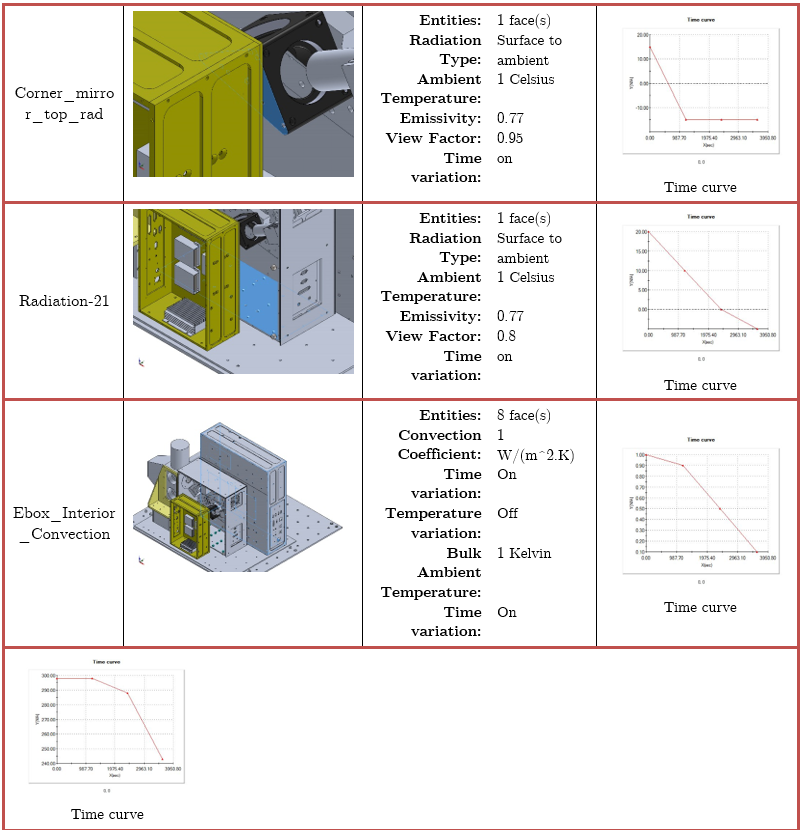
\includegraphics[width=\textwidth]{thermal_load_images/ascent_pt1_TL_images/ascesnt_pt1_11.PNG}
\end{figure}

\begin{figure}
    \centering
    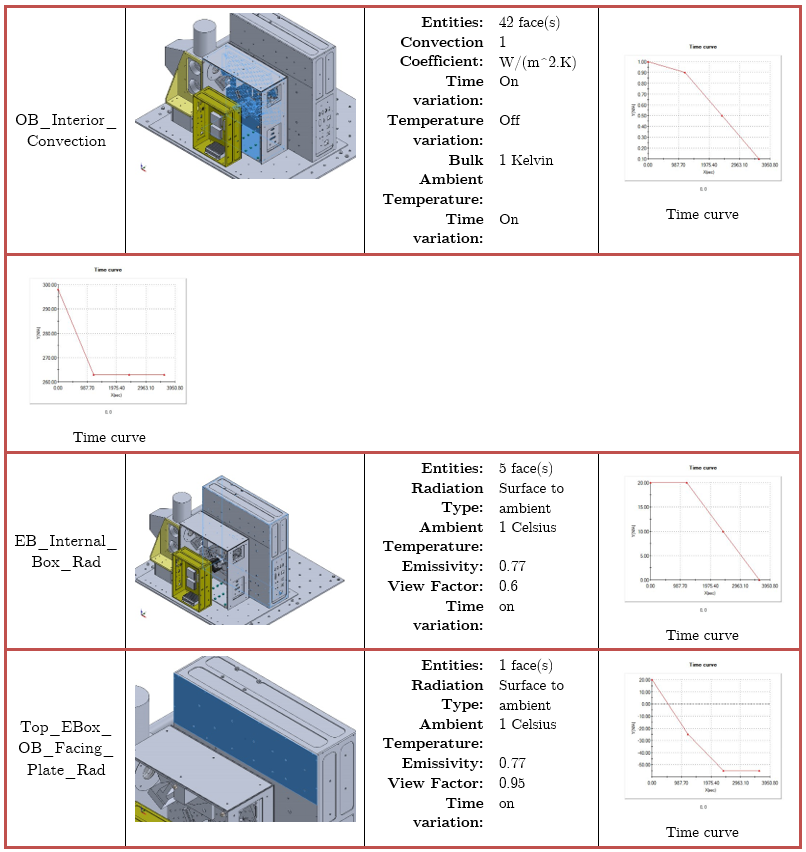
\includegraphics[width=\textwidth]{thermal_load_images/ascent_pt1_TL_images/ascesnt_pt1_12.PNG}
\end{figure}

\begin{figure}
    \centering
    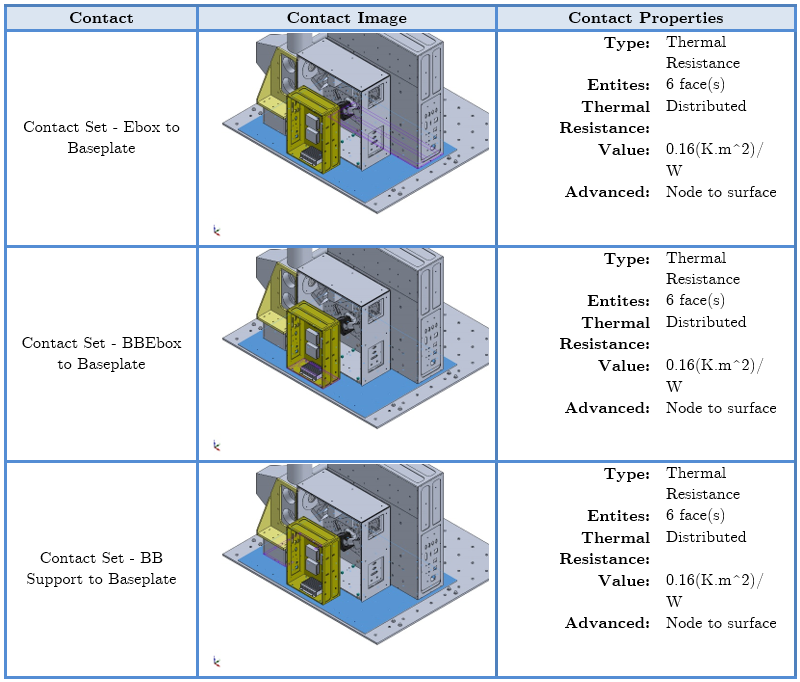
\includegraphics[width=\textwidth]{thermal_load_images/ascent_pt1_TL_images/ascesnt_pt1_13.PNG}
\end{figure}

\begin{figure}
    \centering
    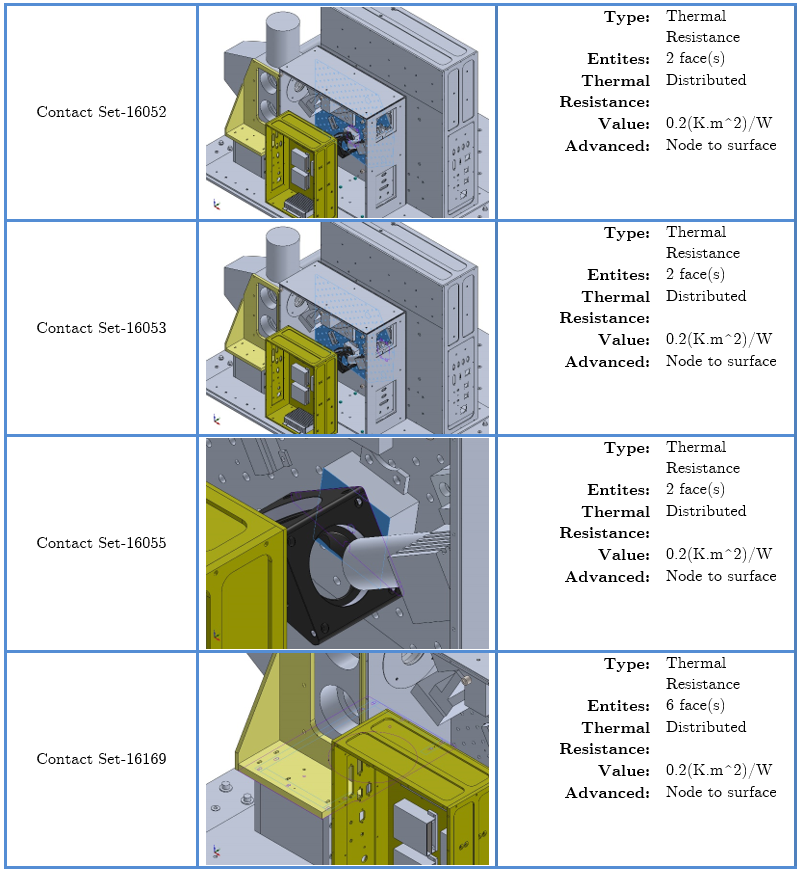
\includegraphics[width=\textwidth]{thermal_load_images/ascent_pt1_TL_images/ascesnt_pt1_14.PNG}
\end{figure}

\begin{figure}
    \centering
    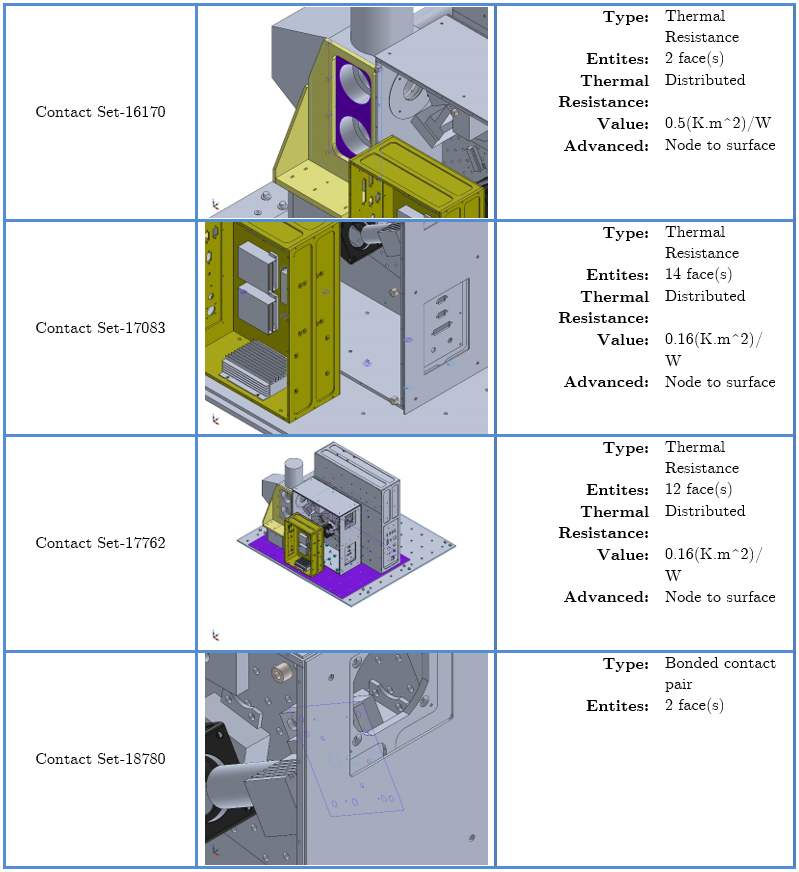
\includegraphics[width=\textwidth]{thermal_load_images/ascent_pt1_TL_images/ascesnt_pt1_15.PNG}
\end{figure}

\begin{figure}
    \centering
    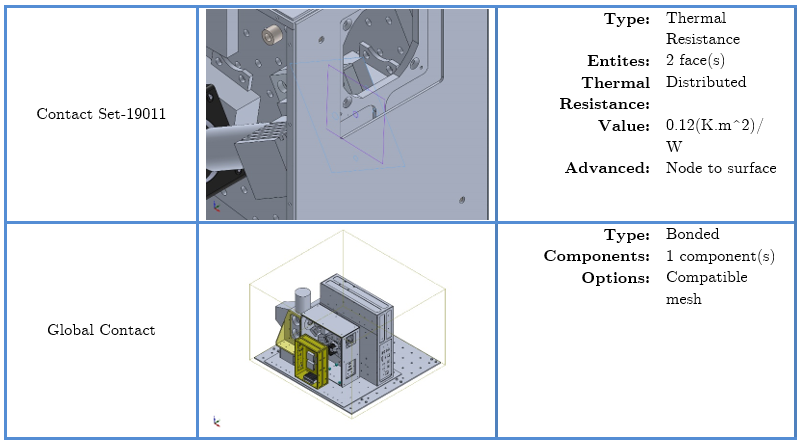
\includegraphics[width=\textwidth]{thermal_load_images/ascent_pt1_TL_images/ascesnt_pt1_16.PNG}
\end{figure}

\clearpage
\section{Ascent Phase: Part 2}

\begin{figure}[h!]
    \centering
    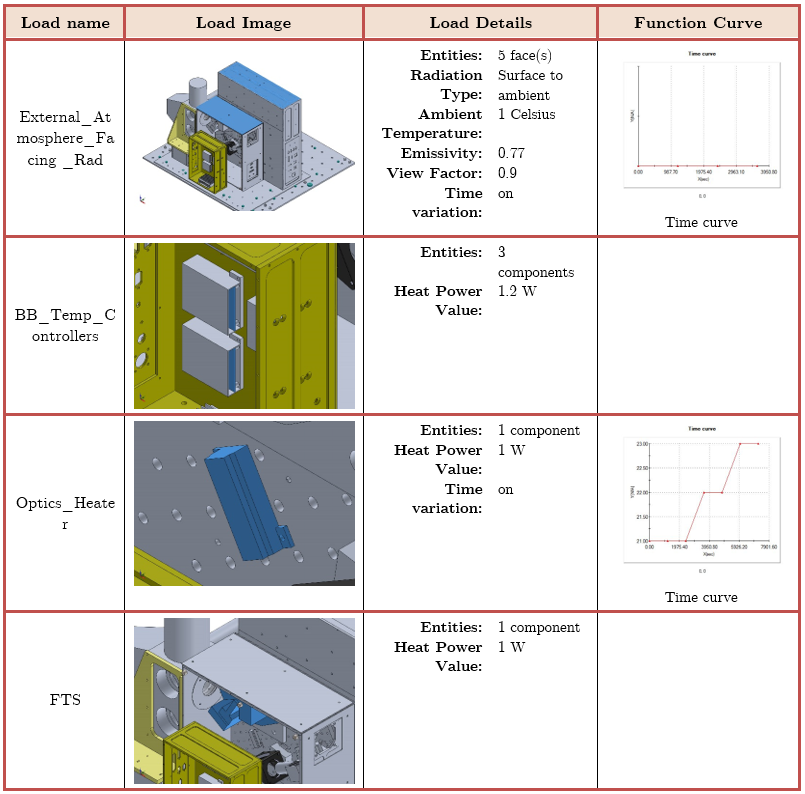
\includegraphics[width=\textwidth]{thermal_load_images/ascent_pt2_TL_images/ascesnt_pt2_1.PNG}
\end{figure}

\begin{figure}
    \centering
    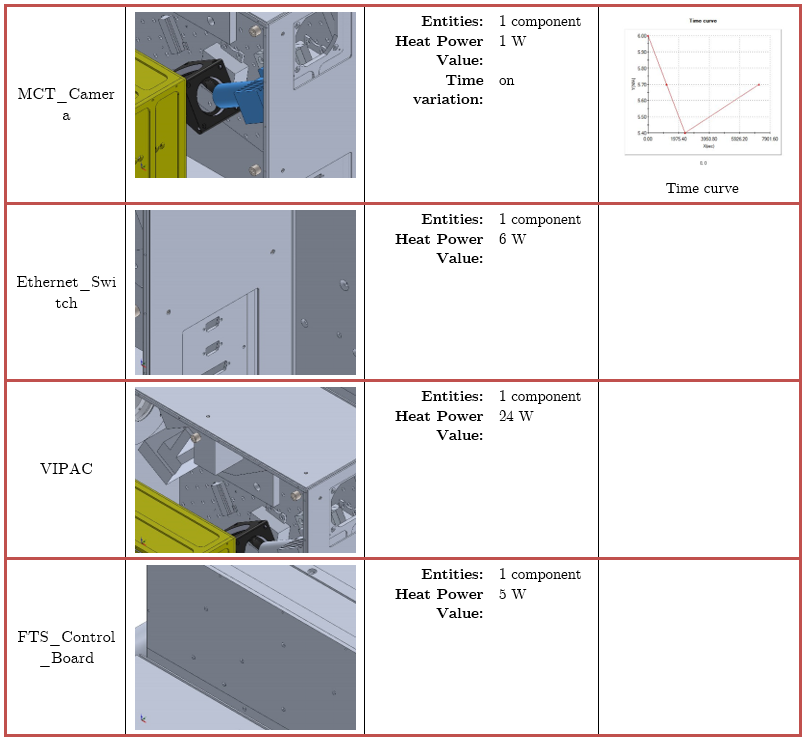
\includegraphics[width=\textwidth]{thermal_load_images/ascent_pt2_TL_images/ascesnt_pt2_2.png}
\end{figure}

\begin{figure}
    \centering
    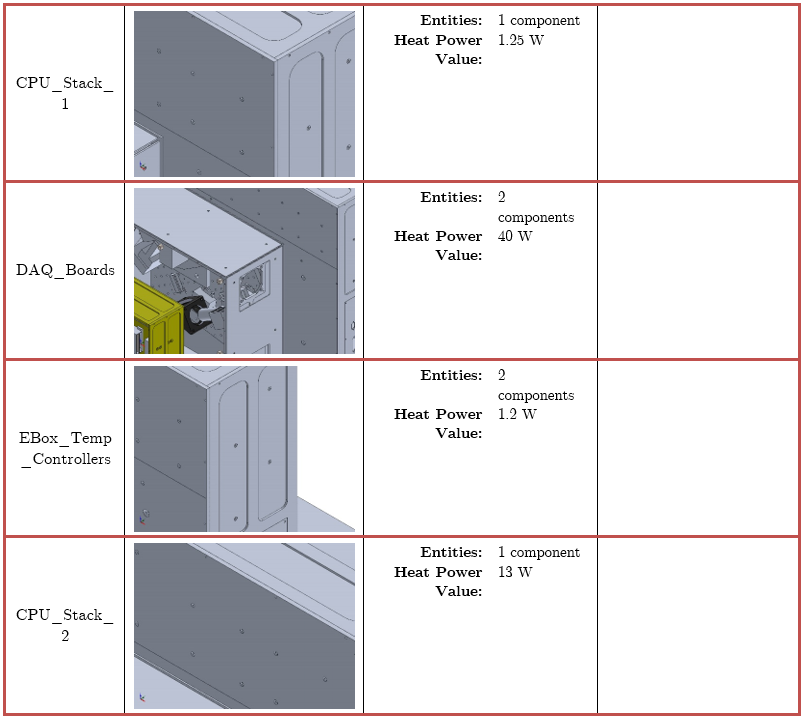
\includegraphics[width=\textwidth]{thermal_load_images/ascent_pt2_TL_images/ascesnt_pt2_3.PNG}
\end{figure}

\begin{figure}
    \centering
    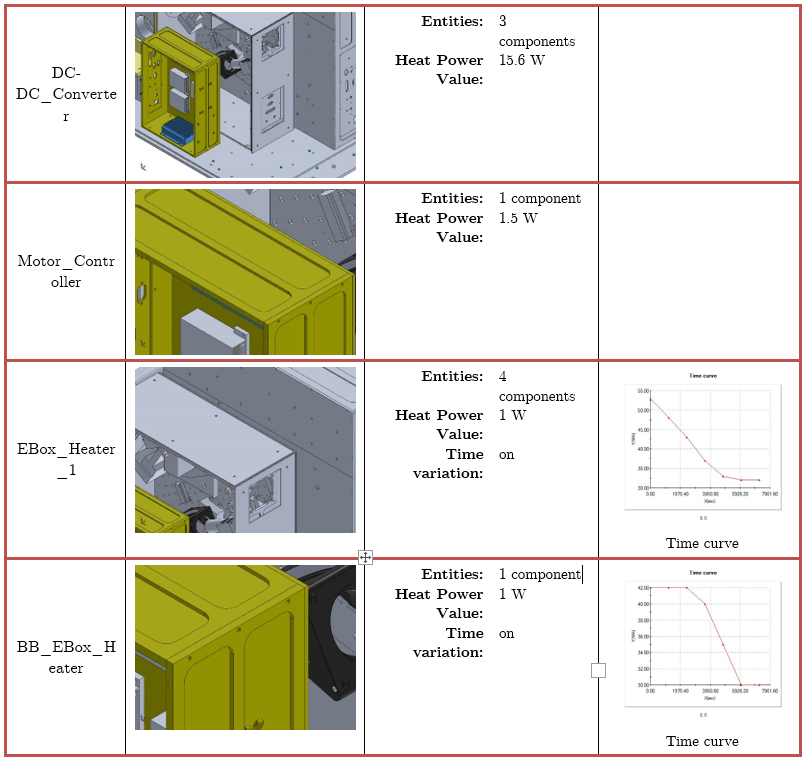
\includegraphics[width=\textwidth]{thermal_load_images/ascent_pt2_TL_images/ascesnt_pt2_4.PNG}
\end{figure}

\begin{figure}
    \centering
    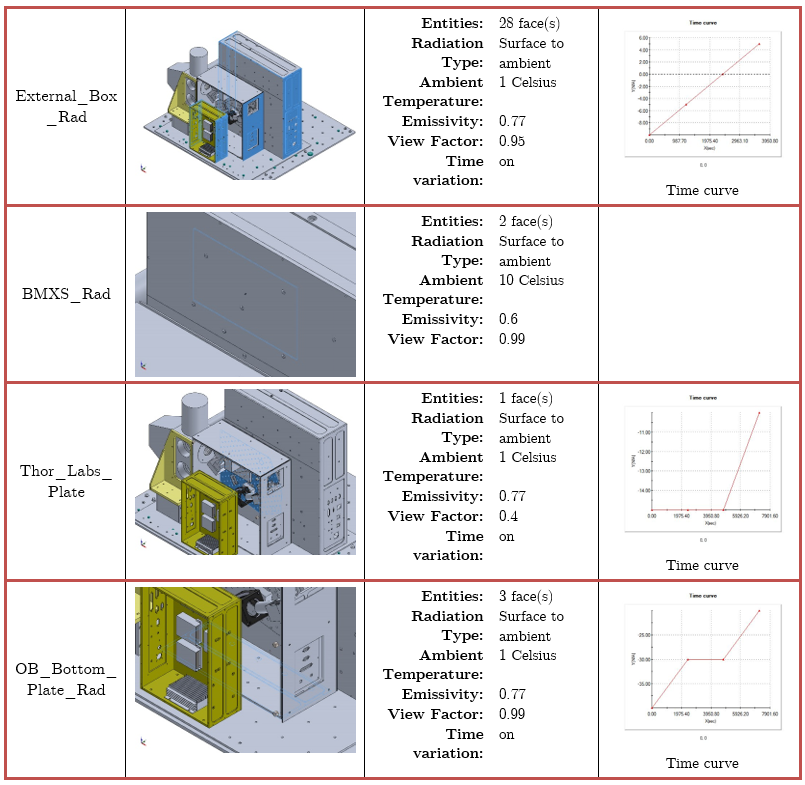
\includegraphics[width=\textwidth]{thermal_load_images/ascent_pt2_TL_images/ascesnt_pt2_5.PNG}
\end{figure}

\begin{figure}
    \centering
    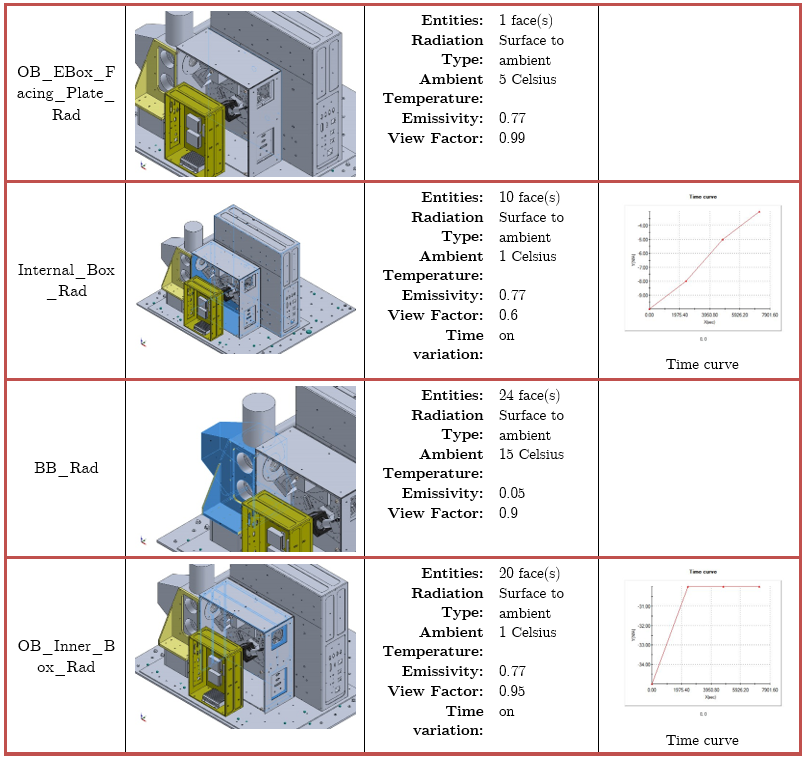
\includegraphics[width=\textwidth]{thermal_load_images/ascent_pt2_TL_images/ascesnt_pt2_6.PNG}
\end{figure}

\begin{figure}
    \centering
    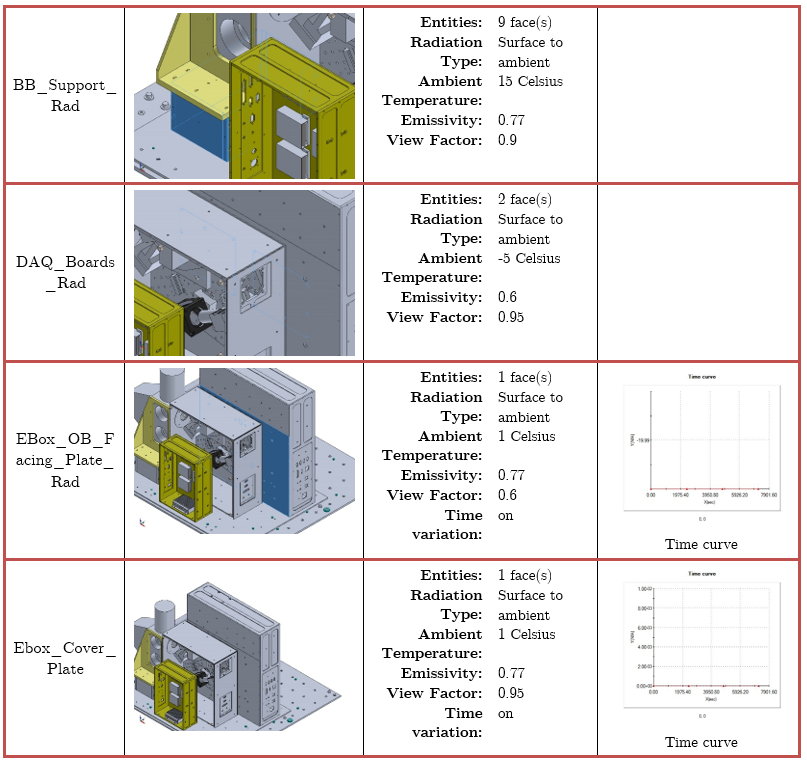
\includegraphics[width=\textwidth]{thermal_load_images/ascent_pt2_TL_images/ascesnt_pt2_7.PNG}
\end{figure}

\begin{figure}
    \centering
    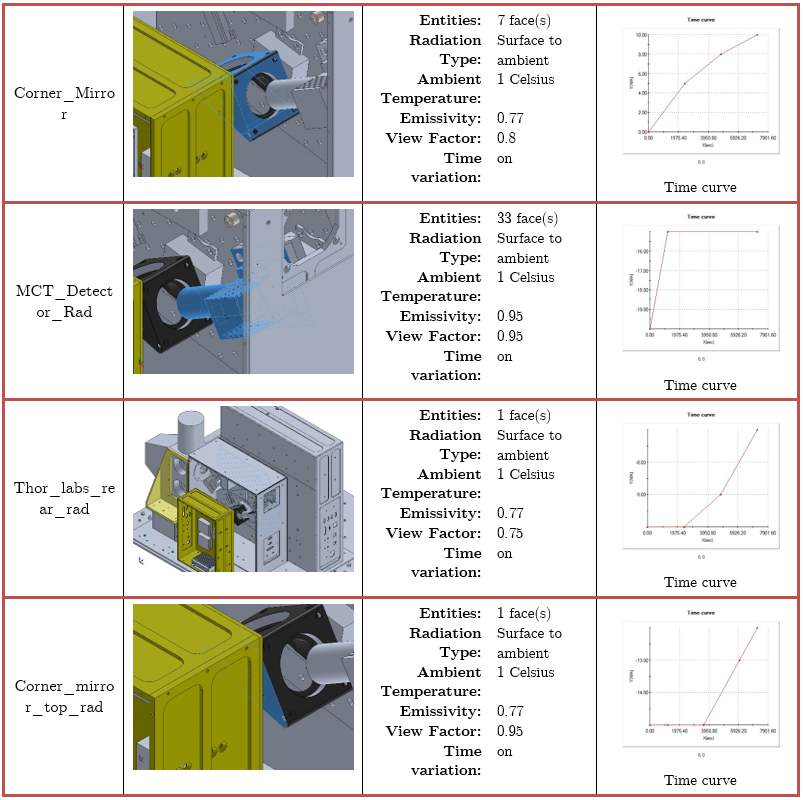
\includegraphics[width=\textwidth]{thermal_load_images/ascent_pt2_TL_images/ascesnt_pt2_8.PNG}
\end{figure}

\begin{figure}
    \centering
    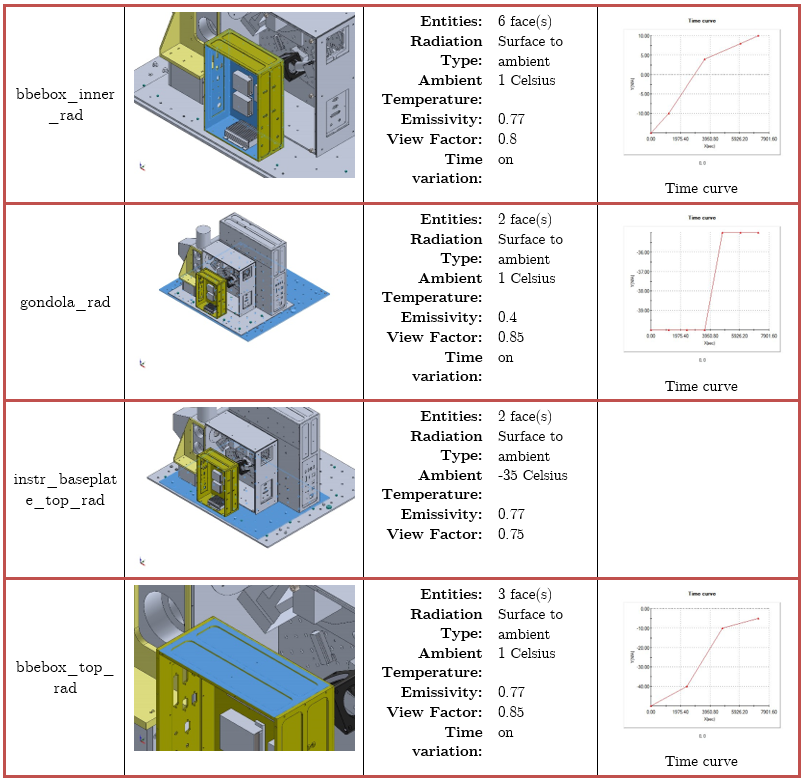
\includegraphics[width=\textwidth]{thermal_load_images/ascent_pt2_TL_images/ascesnt_pt2_9.PNG}
\end{figure}

\begin{figure}
    \centering
    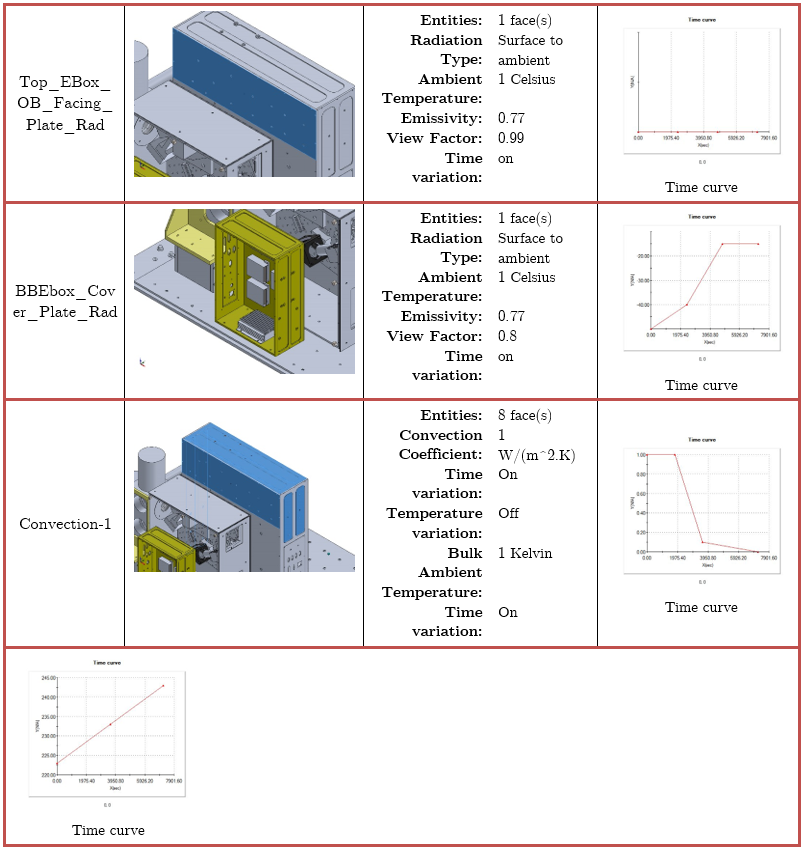
\includegraphics[width=\textwidth]{thermal_load_images/ascent_pt2_TL_images/ascesnt_pt2_10.PNG}
\end{figure}

\begin{figure}
    \centering
    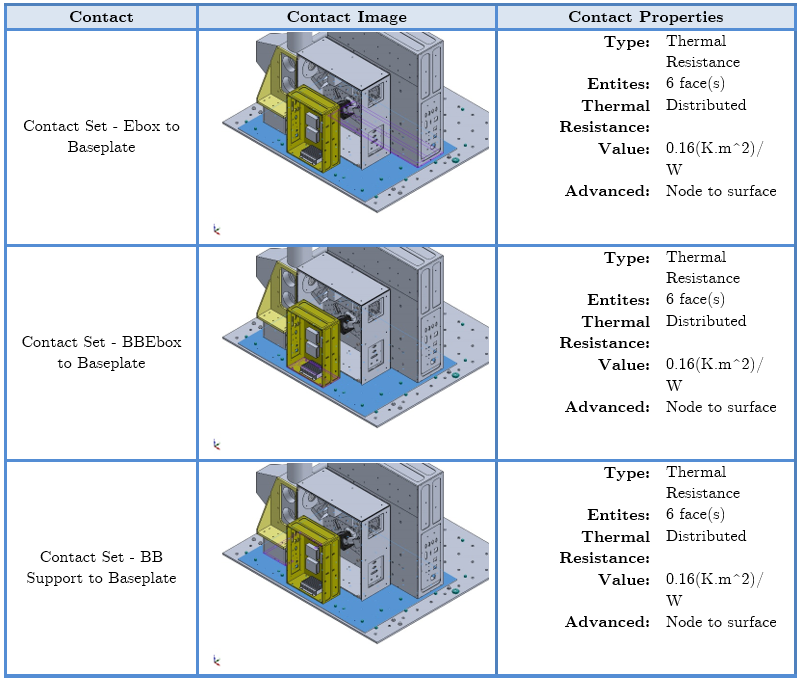
\includegraphics[width=\textwidth]{thermal_load_images/ascent_pt2_TL_images/ascesnt_pt2_11.PNG}
\end{figure}

\begin{figure}
    \centering
    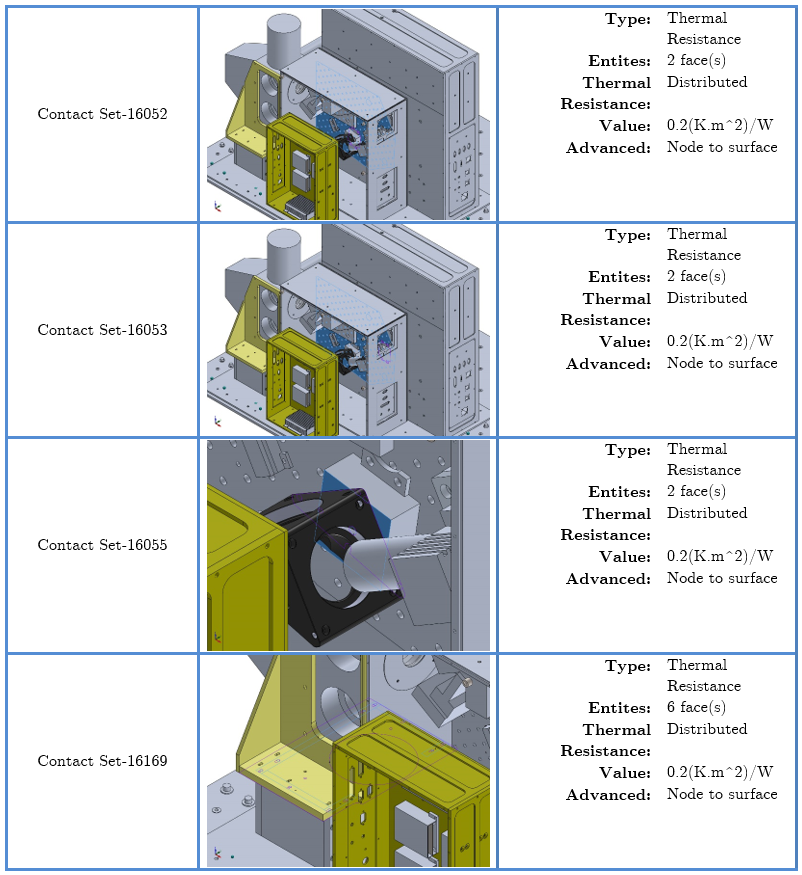
\includegraphics[width=\textwidth]{thermal_load_images/ascent_pt2_TL_images/ascesnt_pt2_12.PNG}
\end{figure}

\begin{figure}
    \centering
    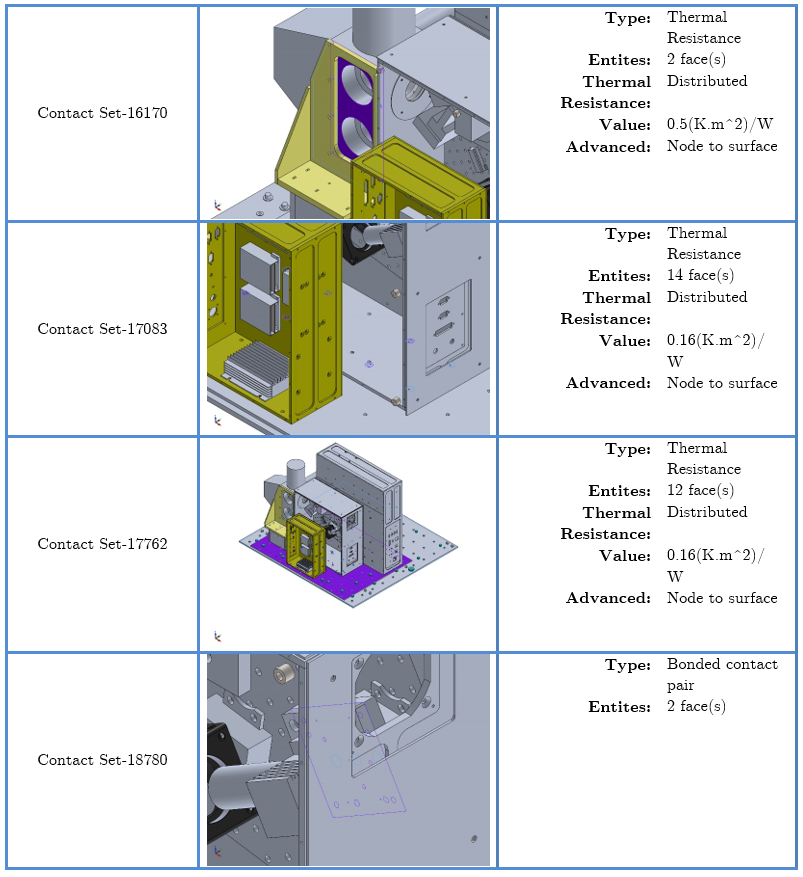
\includegraphics[width=\textwidth]{thermal_load_images/ascent_pt2_TL_images/ascesnt_pt2_13.PNG}
\end{figure}

\begin{figure}
    \centering
    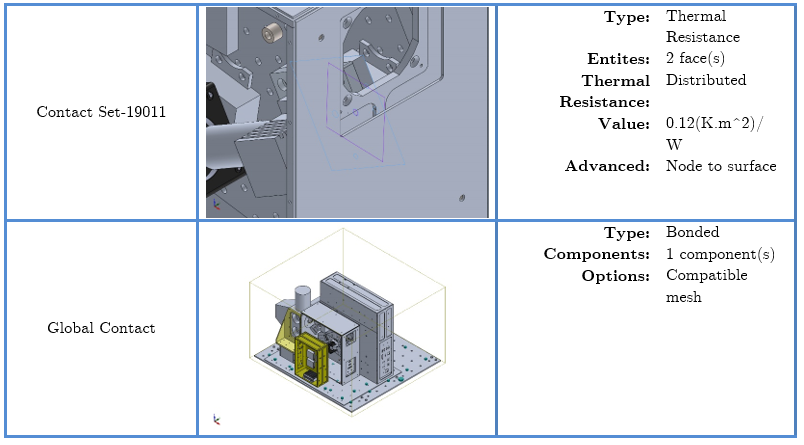
\includegraphics[width=\textwidth]{thermal_load_images/ascent_pt2_TL_images/ascesnt_pt2_14.PNG}
\end{figure}

\clearpage
\section{Float Phase}

\begin{figure}[h!]
    \centering
    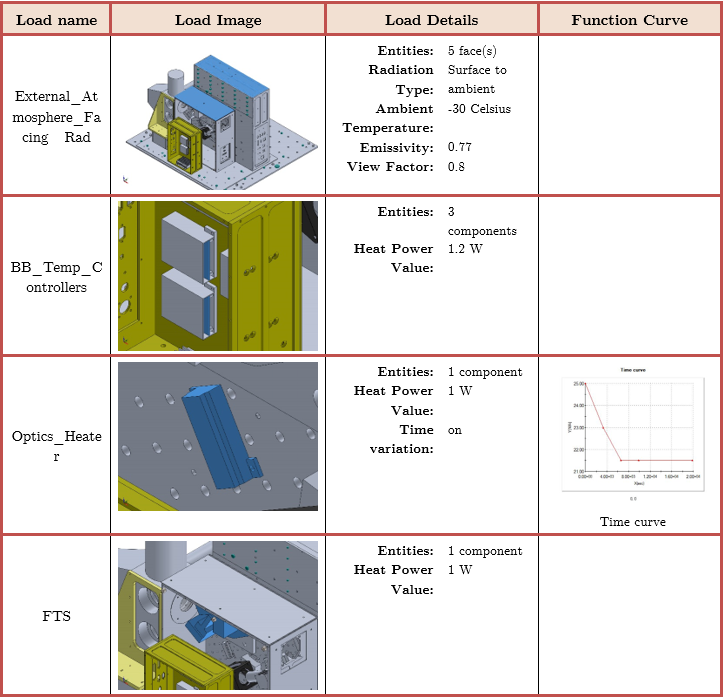
\includegraphics[width=\textwidth]{thermal_load_images/float_TL_images/float_1.PNG}
\end{figure}

\begin{figure}
    \centering
    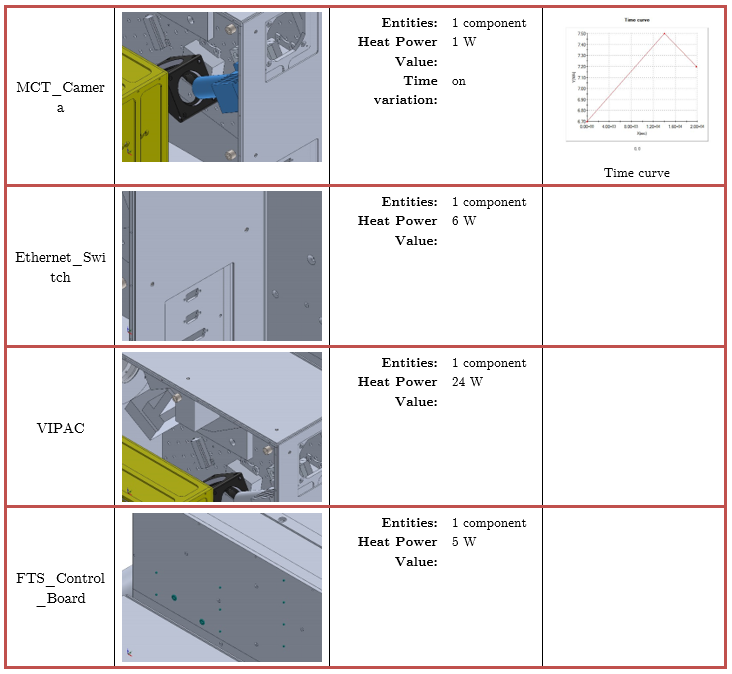
\includegraphics[width=\textwidth]{thermal_load_images/float_TL_images/float_2.PNG}
\end{figure}

\begin{figure}
    \centering
    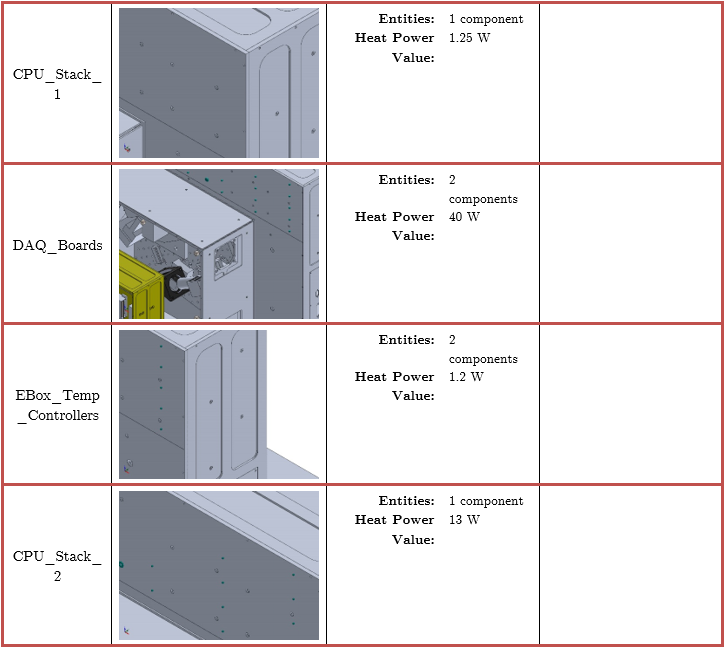
\includegraphics[width=\textwidth]{thermal_load_images/float_TL_images/float_3.PNG}
\end{figure}

\begin{figure}
    \centering
    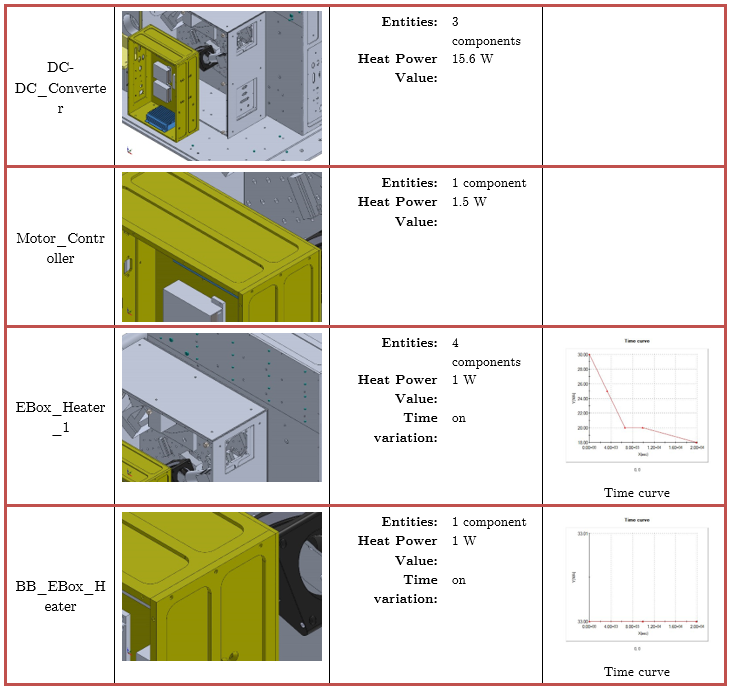
\includegraphics[width=\textwidth]{thermal_load_images/float_TL_images/float_4.PNG}
\end{figure}

\begin{figure}
    \centering
    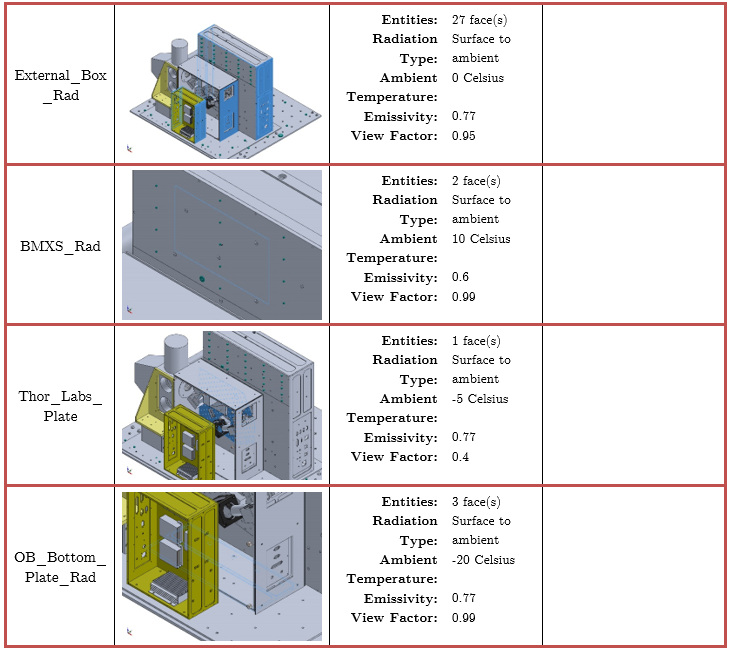
\includegraphics[width=\textwidth]{thermal_load_images/float_TL_images/float_5.PNG}
\end{figure}

\begin{figure}
    \centering
    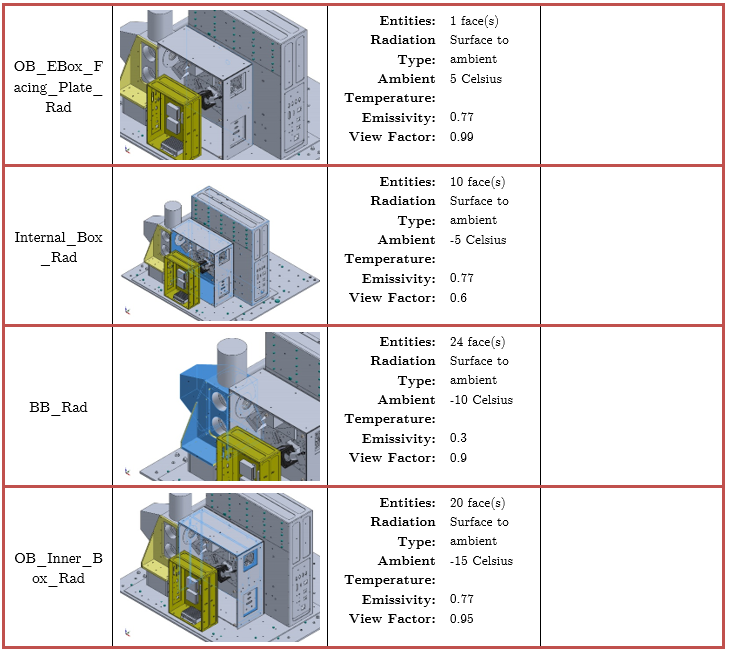
\includegraphics[width=\textwidth]{thermal_load_images/float_TL_images/float_6.PNG}
\end{figure}

\begin{figure}
    \centering
    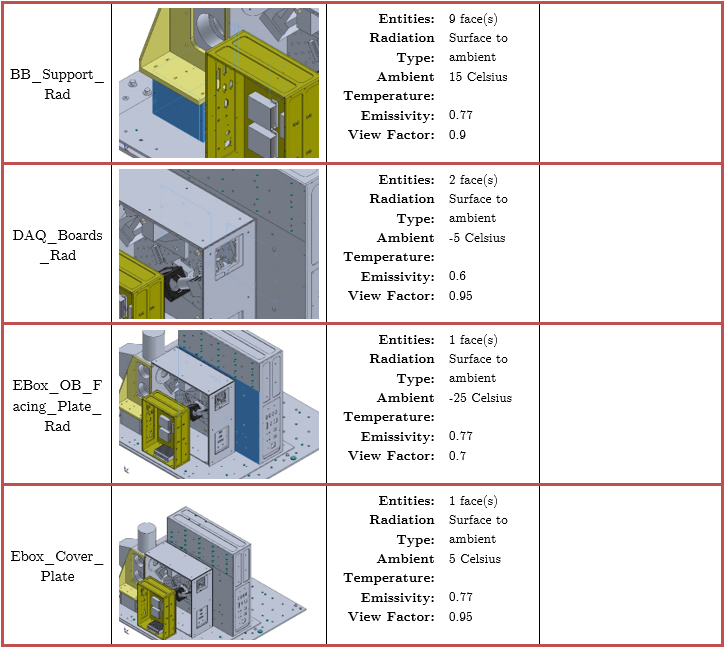
\includegraphics[width=\textwidth]{thermal_load_images/float_TL_images/float_7.PNG}
\end{figure}

\begin{figure}
    \centering
    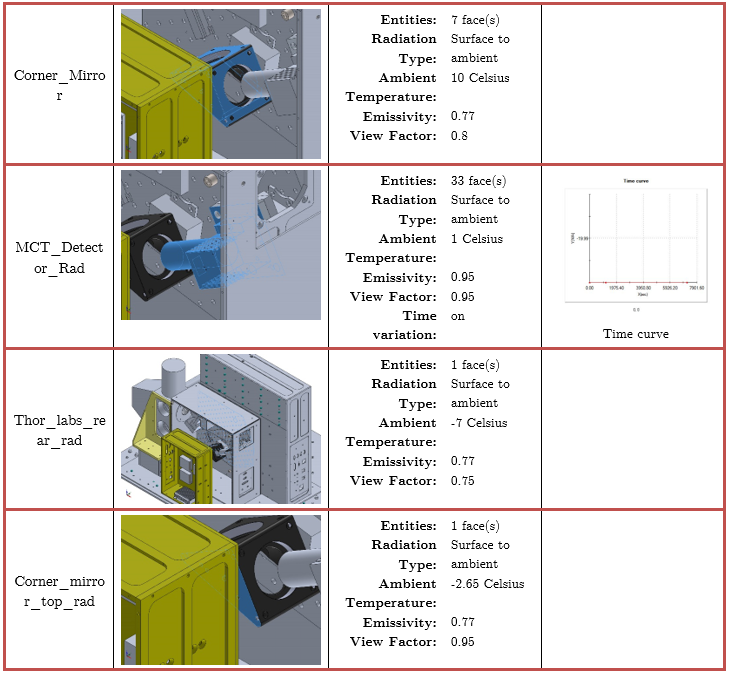
\includegraphics[width=\textwidth]{thermal_load_images/float_TL_images/float_8.PNG}
\end{figure}

\begin{figure}
    \centering
    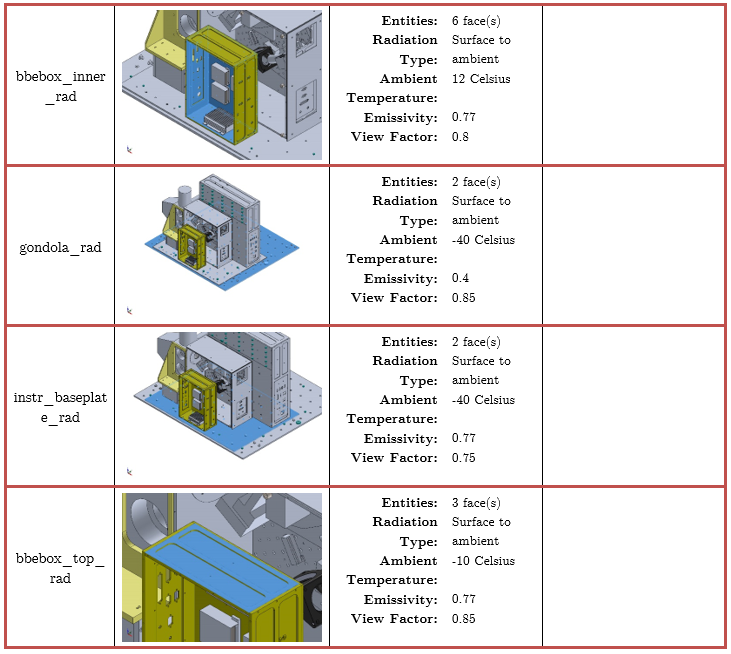
\includegraphics[width=\textwidth]{thermal_load_images/float_TL_images/float_9.PNG}
\end{figure}

\begin{figure}
    \centering
    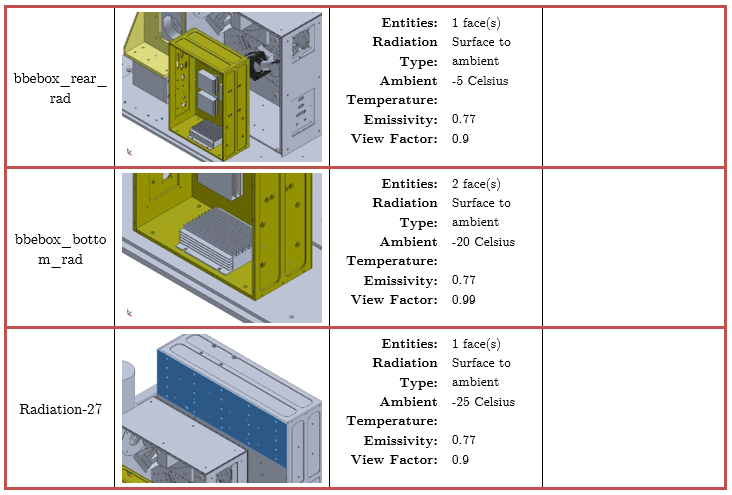
\includegraphics[width=\textwidth]{thermal_load_images/float_TL_images/float_10.PNG}
\end{figure}

\begin{figure}
    \centering
    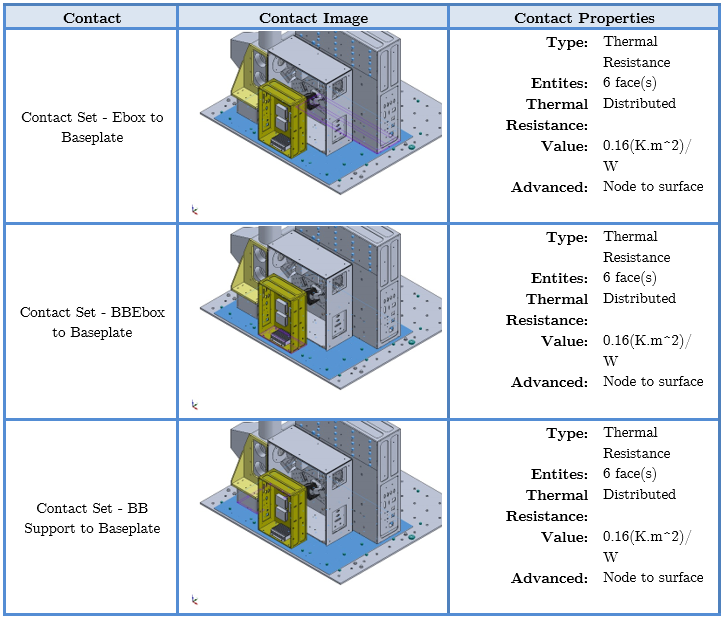
\includegraphics[width=\textwidth]{thermal_load_images/float_TL_images/float_11.PNG}
\end{figure}

\begin{figure}
    \centering
    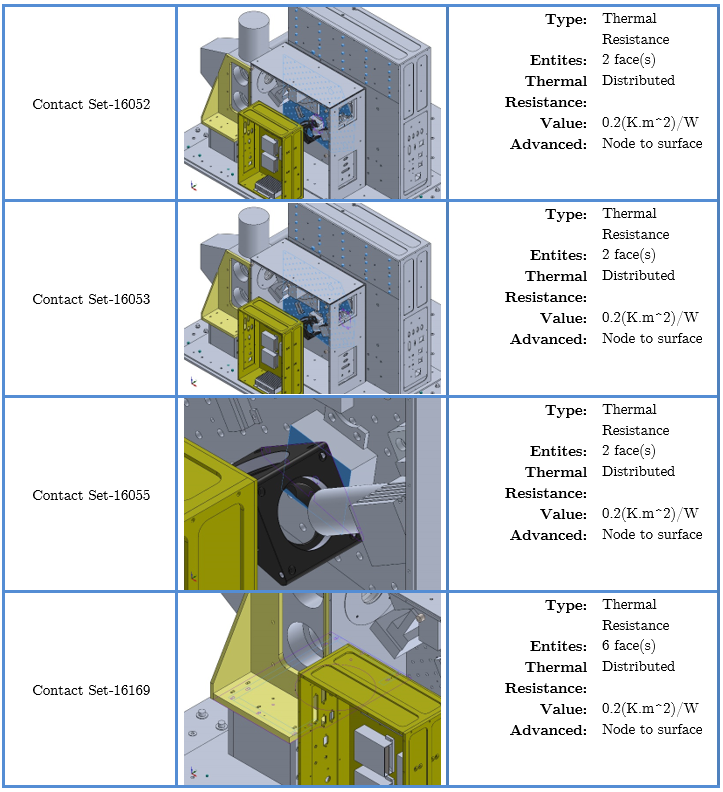
\includegraphics[width=\textwidth]{thermal_load_images/float_TL_images/float_12.PNG}
\end{figure}

\begin{figure}
    \centering
    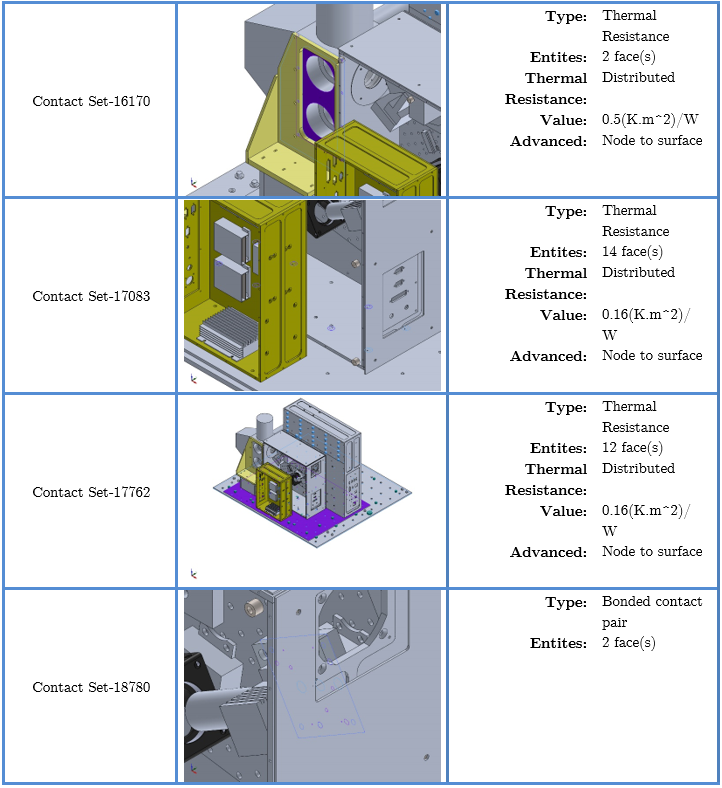
\includegraphics[width=\textwidth]{thermal_load_images/float_TL_images/float_13.PNG}
\end{figure}

\begin{figure}
    \centering
    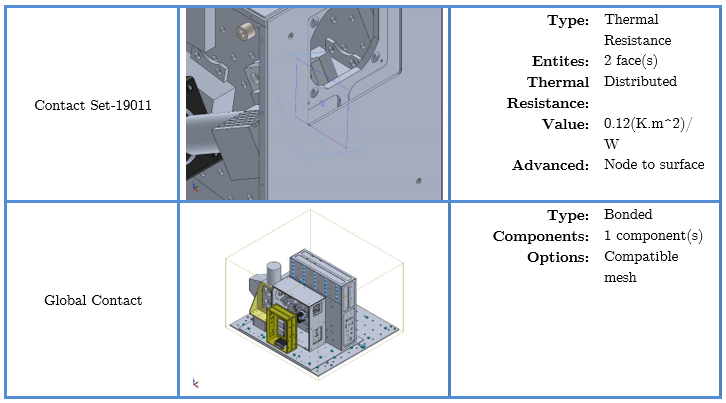
\includegraphics[width=\textwidth]{thermal_load_images/float_TL_images/float_14.PNG}
\end{figure}

\clearpage
\section{Sunrise Phase}

\begin{figure}[h!]
    \centering
    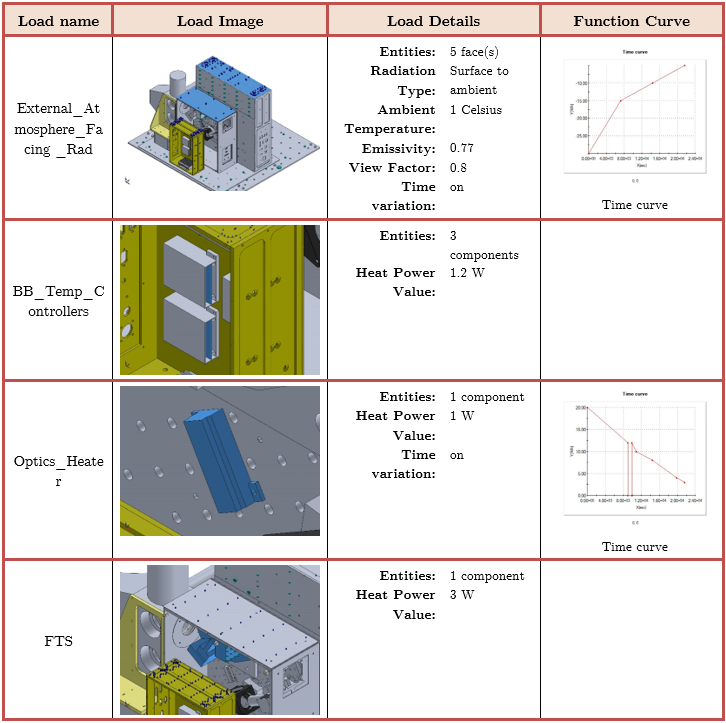
\includegraphics[width=\textwidth]{thermal_load_images/sunrise_TL_images/sunrise_1.PNG}
\end{figure}

\begin{figure}
    \centering
    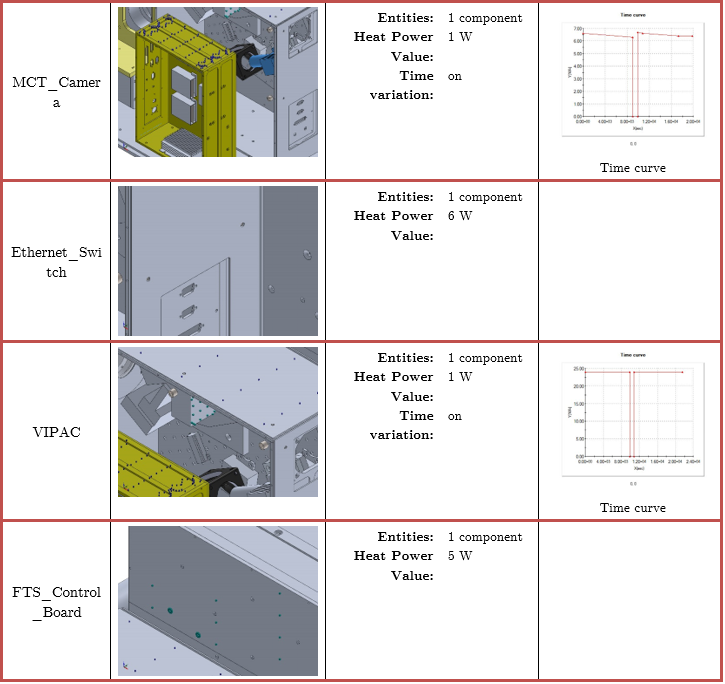
\includegraphics[width=\textwidth]{thermal_load_images/sunrise_TL_images/sunrise_2.PNG}
\end{figure}

\begin{figure}
    \centering
    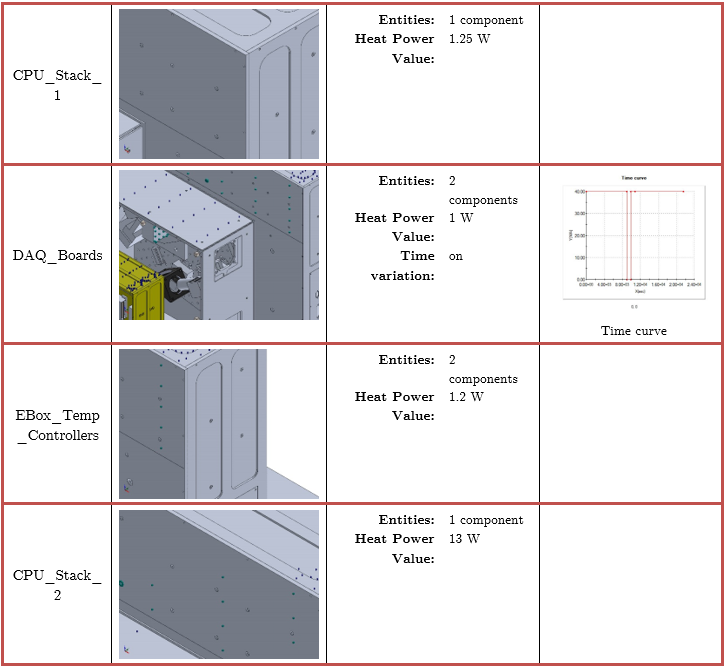
\includegraphics[width=\textwidth]{thermal_load_images/sunrise_TL_images/sunrise_3.PNG}
\end{figure}

\begin{figure}
    \centering
    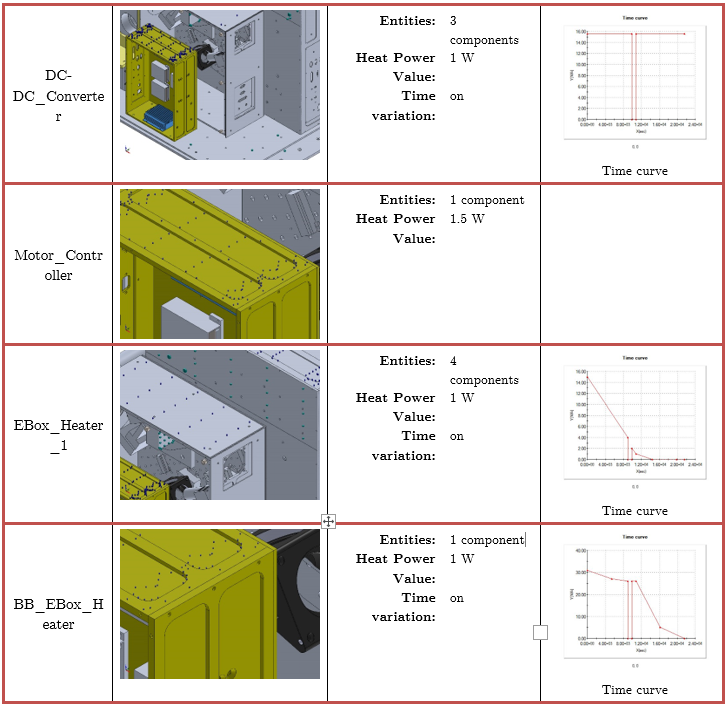
\includegraphics[width=\textwidth]{thermal_load_images/sunrise_TL_images/sunrise_4.PNG}
\end{figure}

\begin{figure}
    \centering
    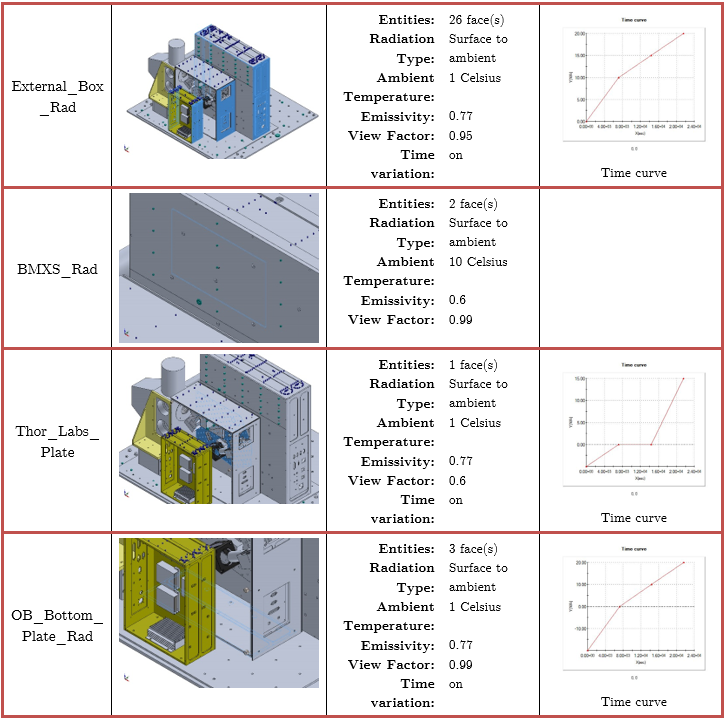
\includegraphics[width=\textwidth]{thermal_load_images/sunrise_TL_images/sunrise_5.PNG}
\end{figure}

\begin{figure}
    \centering
    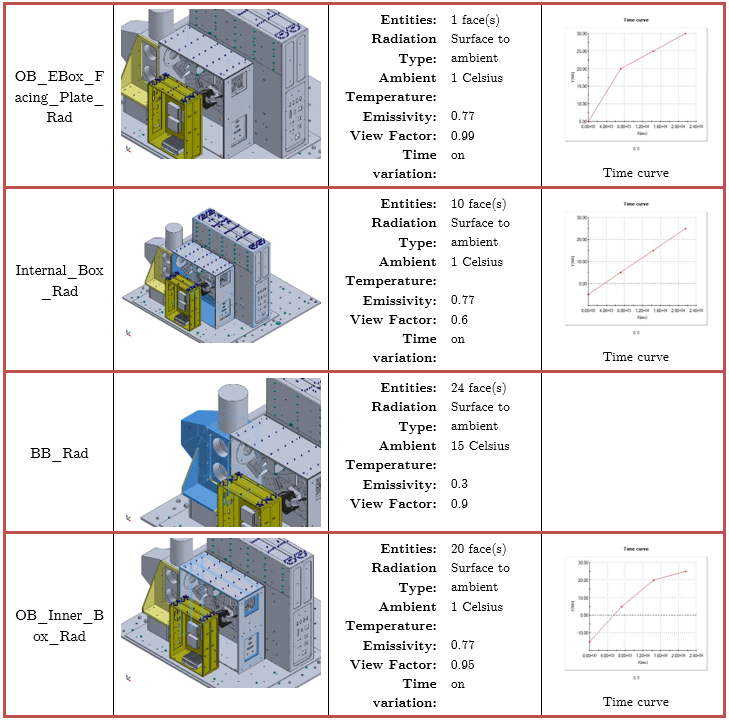
\includegraphics[width=\textwidth]{thermal_load_images/sunrise_TL_images/sunrise_6.PNG}
\end{figure}

\begin{figure}
    \centering
    \includegraphics[width=\textwidth]{thermal_load_images/sunrise_TL_images/sunrise_7.PNG}
\end{figure}

\begin{figure}
    \centering
    \includegraphics[width=\textwidth]{thermal_load_images/sunrise_TL_images/sunrise_8.PNG}
\end{figure}

\begin{figure}
    \centering
    \includegraphics[width=\textwidth]{thermal_load_images/sunrise_TL_images/sunrise_9.PNG}
\end{figure}

\begin{figure}
    \centering
    \includegraphics[width=\textwidth]{thermal_load_images/sunrise_TL_images/sunrise_10.PNG}
\end{figure}

\begin{figure}
    \centering
    \includegraphics[width=\textwidth]{thermal_load_images/sunrise_TL_images/sunrise_11.PNG}
\end{figure}

\begin{figure}
    \centering
    \includegraphics[width=\textwidth]{thermal_load_images/sunrise_TL_images/sunrise_12.PNG}
\end{figure}

\begin{figure}
    \centering
    \includegraphics[width=\textwidth]{thermal_load_images/sunrise_TL_images/sunrise_13.PNG}
\end{figure}

\begin{figure}
    \centering
    \includegraphics[width=\textwidth]{thermal_load_images/sunrise_TL_images/sunrise_14.PNG}
\end{figure}

\begin{figure}
    \centering
    \includegraphics[width=\textwidth]{thermal_load_images/sunrise_TL_images/sunrise_15.PNG}
\end{figure}